\chapter{Anhang}
\label{kap:anhang}

\section{Reproduktion}

\begin{footnotesize}
\begin{verbatim}
# 0  Sichtung (erzeugt alle Messwerte aus Kapitel 4)
python src/analyze_data.py
# 1  Objektausschnitte freistellen  -> assets/masks/
python src/matting.py
# 2  Okkluder-Bibliothek            -> assets/bars/
python src/occluders.py
# 3  Trainingsdaten                 -> synth/train/ + generation_report.json
python src/generate.py --out synth/train --n 6000 --seed 1 --preview 8
python src/generate.py --out synth/sval  --n  400 --seed 99
# 4  Training
python src/train.py --name baseline
# 5  Auswertung (eigene Metriken + Kreuzvergleich)
python src/evaluate.py --weights runs/baseline/weights/best.pt \
    --splits val,test --crosscheck --out docs/experiments/final_eval.json
# 6  Auflösungssweep und Experiment
python src/experiment.py infer          # Sweep (Abschnitt 7.3)
python src/experiment.py ablation-data  # Experiment  (Abschnitt 7.4)
python src/experiment.py ablation-train
python src/experiment.py ablation-eval
# 7  Diagramme und Tabellen
python src/report.py
python paper/tools/fig_boxversatz.py
python paper/tools/fig_qual_iou.py
python paper/tools/fig_stufen.py
python paper/tools/abbildungen_vorbereiten.py
\end{verbatim}
\end{footnotesize}

Eine Einschränkung der Ausführungsumgebung erzwingt einen Trainingsparameter: In
der verwendeten Kombination aus \code{opencv-python}~5.0.0.93 und
\code{torch}~2.13 verklemmt sich der fork-basierte DataLoader reproduzierbar beim
ersten Batch, sobald \code{workers > 0} gesetzt ist -- unabhängig von
\code{cv2.setNumThreads(0)}, deaktiviertem OpenCL, gesetzten Thread-Limits oder
der Startmethode \code{spawn}. Das Training läuft deshalb mit \code{workers=0}
und hält stattdessen alle dekodierten Bilder im Arbeitsspeicher
(\code{cache='ram'}, etwa 18\,GB); der Cache wird von einem Thread-Pool gefüllt
und ist vom Deadlock nicht betroffen.

\section{Gemessene Anteile aus dem Erzeugungsbericht}

Die folgenden Werte stammen unverändert aus
\code{synth/train/generation\_report.json} und sind die Belegquelle für alle
Ist-Anteile in Tabelle~\ref{tab:parameter}.

\begin{footnotesize}
\begin{verbatim}
n_images                      6000        instances_rendered      173100
canvas                        1024        instances_labeled       136384
boxes_per_image_mean          22.73       dropped_occluded         30801
mean_visibility_all_rendered   0.7569     dropped_offscreen         3846
mean_visibility_labeled        0.9002     dropped_tiny               228

inst_rotation      (je Instanz)  1.0000    negative_image  (je Bild)  0.0973
inst_oval          (je Instanz)  0.5707    img_has_bars    (je Bild)  0.5835
inst_dent          (je Instanz)  0.1814    img_clutter     (je Bild)  0.3157
inst_perspective   (je Instanz)  0.3020    recess          (je Bild)  0.8738
inst_photometric   (je Instanz)  0.9976    bg_fliplr       (je Bild)  0.5047
inst_gamma         (je Instanz)  0.7969    bg_flipud       (je Bild)  0.1487
inst_hsv           (je Instanz)  0.6973    bg_rot          (je Bild)  0.3428
inst_harmonize     (je Instanz)  0.8482    glob_bc         (je Bild)  0.8958
inst_blur          (je Instanz)  0.5983    glob_hsv        (je Bild)  0.6897
inst_noise         (je Instanz)  0.6988    glob_blur       (je Bild)  0.3435
inst_shadow        (je Instanz)  0.4931    glob_motion     (je Bild)  0.0988
inst_stub          (je Instanz)  0.8801    glob_noise      (je Bild)  0.8015
inst_occluded (je Label)         0.3009    glob_vignette   (je Bild)  0.2502
\end{verbatim}
\end{footnotesize}

Ein Wert ist nicht als Anteil lesbar: \code{recess} zählt die \emph{Anzahl} der
abgedunkelten Mulden je Bild. Der Sollwert ist 0,55 je Cluster, die erwartete
Clusterzahl beträgt
$0{,}45 \cdot 1 + 0{,}35 \cdot 2 + 0{,}20 \cdot 3 = 1{,}75$, und unter
Berücksichtigung der 9,7\,\% Negativbilder ergibt sich
$0{,}55 \cdot 1{,}75 \cdot 0{,}903 = 0{,}869$ -- was den gemessenen Wert 0,8738
erklärt. \code{img\_has\_bars} ist dagegen ein echter Anteil; der Sollwert 0,65
reduziert sich durch die Negativbilder auf $0{,}65 \cdot 0{,}903 = 0{,}587$ und
trifft den gemessenen Wert 0,5835.

\section{Vollständiger Sweep der Inferenzauflösung}

Tabelle~\ref{tab:imgszvoll} ergänzt den Auszug aus
Abschnitt~\ref{sec:imgsz} um die fehlenden Stufen.

\begin{table}[htbp]
\centering
\caption[Vollständiger Auflösungssweep]{Vollständiger Sweep der
Inferenzauflösung für die yolo11s-Baseline.}
\label{tab:imgszvoll}
\footnotesize
\begin{tabular}{@{}lrrrrrr@{}}
\toprule
\code{imgsz} & \multicolumn{3}{c}{\code{val}} & \multicolumn{3}{c}{\code{test}} \\
 & \mAPfifty{} & \mAPall{} & $F_1$ & \mAPfifty{} & \mAPall{} & $F_1$ \\
\midrule
640  & 0,435 & 0,201 & 0,507 & 0,512 & 0,325 & 0,606 \\
800  & 0,793 & 0,428 & 0,768 & 0,642 & 0,351 & 0,685 \\
960  & 0,852 & 0,498 & 0,840 & 0,881 & 0,428 & 0,852 \\
1024 & 0,868 & 0,546 & 0,876 & 0,879 & 0,468 & 0,847 \\
1280 & 0,887 & 0,577 & 0,861 & 0,917 & 0,469 & 0,917 \\
1600 & 0,904 & 0,606 & 0,850 & 0,956 & 0,466 & 0,971 \\
1920 & 0,893 & 0,613 & 0,851 & 0,956 & 0,479 & 0,959 \\
2240 & 0,880 & 0,588 & 0,843 & 0,944 & 0,484 & 0,930 \\
2464 & 0,886 & 0,597 & 0,862 & 0,941 & 0,478 & 0,947 \\
\bottomrule
\end{tabular}
\end{table}

\section{Sensitivität gegenüber dem Größenversatz}

Die Rechnung zu Abschnitt~\ref{sec:boxversatz} (1,15\px{} je Seite auf
\code{test}, 0,58\px{} auf \code{val}): Alle vorhergesagten Boxen werden
um den gemessenen medianen Fehlbetrag je Seite aufgeweitet (1,27\px{} auf
\code{test}, 0,58\px{} auf \code{val}) und neu ausgewertet.

\begin{table}[htbp]
\centering
\caption[Sensitivität gegenüber dem Größenversatz]{Sensitivitätsrechnung: alle
vorhergesagten Boxen um den medianen Fehlbetrag je Seite aufgeweitet. Das ist
\emph{kein} Ergebnis eines neuen Trainings, sondern eine Obergrenzenschätzung für
den Effekt einer angeglichenen Labelkonvention.}
\label{tab:boxsens}
\footnotesize
\begin{tabular}{@{}llrrrrr@{}}
\toprule
\textbf{Split} & & \mAPfifty{} & \mAPseven{} & \mAPall{} &
\textbf{bestes $F_1$} & \textbf{mittl.\ IoU} \\
\midrule
\code{test} & unverändert       & \textbf{0,956} & 0,326 & 0,466 & \textbf{0,971} & 0,746 \\
\code{test} & Boxen aufgeweitet & 0,936 & \textbf{0,752} &
\textbf{0,617} & 0,948 & \textbf{0,815} \\
\addlinespace
\code{val}  & unverändert       & 0,886 & 0,793 & 0,597 & 0,862 & 0,824 \\
\code{val}  & Boxen aufgeweitet & 0,886 & 0,812 & 0,622 & 0,862 & 0,835 \\
\bottomrule
\end{tabular}
\end{table}

\section{Verfahrensklassen der Bildaugmentierung}

\begin{table}[htbp]
\centering
\caption[Verfahrensklassen der Bildaugmentierung]{Verfahrensklassen der
Bildaugmentierung und ihr Einsatz im vorliegenden Fall.}
\label{tab:taxonomie}
\footnotesize
\begin{tabularx}{\textwidth}{@{}L{0.19\textwidth}X@{}}
\toprule
\textbf{Klasse} & \textbf{Einsatz hier} \\
\midrule
geometrisch, bildweit \newline
\scriptsize\cite{krizhevsky2012}; \cite{simard2003} &
Spiegelung, Skalierung, Translation: ja. Rotation, Scherung und Perspektive
bildweit: nein -- Labelrauschen (Abschnitt~\ref{sec:boxrotation}) \\
\addlinespace
geometrisch, pro Instanz \newline
\scriptsize\cite{dwibedi2017}; \cite{ghiasi2021} &
ja, im Generator mit exakter Neuberechnung der Box aus der Alphamaske \\
\addlinespace
photometrisch \newline
\scriptsize\cite{krizhevsky2012}; \cite{grossberg2003} &
ja, zweistufig -- pro Instanz und global \\
\addlinespace
Degradation \newline
\scriptsize\cite{hendrycks2019} &
ja (Unschärfe, Rauschen, JPEG); hier zusätzlich als Mittel gegen
Einfügeartefakte (Abschnitt~\ref{sec:shortcut}) \\
\addlinespace
Informationsentzug \newline
\scriptsize\cite{devries2017cutout}; \cite{zhong2020erasing};
\cite{singh2017hideseek} &
nicht in generischer Form; ersetzt durch physikalisch motivierte Verdeckung mit
berechneter Sichtbarkeit (Tabelle~\ref{tab:parameter}, T6) \\
\addlinespace
Mehrbild-Mischung \newline
\scriptsize\cite{zhang2018mixup}; \cite{yun2019cutmix}; \cite{bochkovskiy2020} &
nur Mosaic; mixup und CutMix aus \\
\addlinespace
Synthese \newline
\scriptsize\cite{dvornik2018}; \cite{tobin2017}; \cite{tremblay2018} &
ja -- Kern des Verfahrens (Abschnitt~\ref{sec:augsynthese}) \\
\bottomrule
\end{tabularx}
\end{table}

\section{Alle Transformationen der Synthese-Pipeline}

{\footnotesize
\begin{longtable}{@{}L{0.195\textwidth}L{0.065\textwidth}L{0.55\textwidth}L{0.022\textwidth}@{}}
\caption[Alle Transformationen der Pipeline]{Alle 36 Transformationen der
Pipeline mit Parameterbereich, gemessenem Ist-Anteil und Begründung. \emph{S}
verweist auf die geschlossene Abkürzung aus Abschnitt~\ref{sec:shortcut},
\emph{Art} auf die Belegart wie in Tabelle~\ref{tab:befunde}: \emph{M} = Messung
an den Realdaten, \emph{P} = physikalische Randbedingung, \emph{L} = in der
Literatur belegtes Argument -- die Quelle steht dann in derselben Zeile --,
\emph{A} = Annahme. \emph{P} begründet dabei die \emph{Randbedingung}, also
welche Konfigurationen überhaupt möglich sind, und nur in zwei Fällen (volle
Rotation, horizontale Spiegelung) über eine Symmetrie auch die Verteilung
selbst; wo sie den Parameterwert nicht festlegt, steht \emph{P/A}.}
\label{tab:parameter}\\
\toprule
\textbf{Transformation} & \textbf{Ist} & \textbf{Begründung} & \textbf{Art} \\
\midrule
\endfirsthead
\multicolumn{4}{@{}l}{\itshape Fortsetzung von Tabelle~\ref{tab:parameter}}\\
\toprule
\textbf{Transformation} & \textbf{Ist} & \textbf{Begründung} & \textbf{Art} \\
\midrule
\endhead
\bottomrule
\endfoot
\multicolumn{4}{@{}l}{\textbf{T1 -- Hintergrund} \hfill\emph{Anteile je Bild}}\\
Clean Plate statt Fremdszene & 80\,\%$^\ast$ & Die vier Clean Plates sind exakt die Zieldomäne (Befund~3); die Fremdszenen liefern Kontextvielfalt und harte Negative. Wirksam sind je Clean Plate 20\,\% gegen 6,7\,\% je Fremdszene, also ein dreifaches Gewicht. \textbf{Die Aufteilung 80/20 ist gesetzt} -- eine reale Häufigkeit, an der sie sich messen ließe, gibt es nicht. & M/A \\
Zoom an Rohr-\Oe{} gekoppelt, Gl.~\eqref{eq:zoom} & 100\,\% & Eine Stirnfläche hat zwangsläufig den Durchmesser des Schafts daneben; ein Missverhältnis trainierte eine falsche Kontext-Größen-Relation an. & P \\
Zufallsausschnitt (Translation) & 100\,\% & Bei nur sieben Quellbildern die wichtigste Quelle von Hintergrundvielfalt; zufällige Ausschnitte sind dafür die etablierte Standardaugmentierung \parencite{krizhevsky2012}. & L \\
Reflect-Padding, max.\ $1{,}35\times$ kürzeste Kante & bei Bedarf & Kachelung erzeugte harte achsparallele Nähte; gespiegeltes Padding hat keine Kante. \textbf{Eigene Beobachtung}, für diese Wahl liegt kein Literaturbeleg vor -- und sie ist nicht folgenlos, siehe Abschnitt~\ref{sec:grenzen}. & A \\
horizontale Spiegelung & 50,5\,\% & Label-exakt und physikalisch korrekt: Ein Stapel wird von beiden Enden fotografiert. & P \\
vertikale Spiegelung & 14,9\,\% & Ebenfalls label-exakt, bewusst seltener -- die Schwerkraft erzeugt eine schwache Vorzugsrichtung. & A \\
Kleinrotation $\pm6^\circ$ (Zoom 1,06) & 34,3\,\% & Die Rohrlinien sind nie exakt achsparallel: Der Struktur-Tensor misst für die vier Clean Plates $+0{,}9$, $-1{,}6$, $+0{,}9$ und $+6{,}6$ Grad (Abschnitt~\ref{sec:matting}), was den Bereich setzt. Wirkt vor dem Einfügen, betrifft also keine Boxen. & M \\
\addlinespace
\multicolumn{4}{@{}l}{\textbf{T2 -- Instanzgeometrie} \hfill\emph{Anteile je gerenderter Instanz}}\\
Rotation $0$--$360^\circ$ & 100\,\% & Rohrenden haben keine kanonische Orientierung -- die einzige Orientierungsinformation ist das Glanzlicht, und dessen Richtung hängt vom Sonnenstand ab. Volle Rotationsinvarianz ist korrekt \emph{und} kostenlos, daher 100\,\% statt eines Bruchteils. & P \\
Skalierung auf 12--44\px, Gl.~\eqref{eq:oval} & 100\,\% & Realmessung 12,2--35,8\px{} plus 25\,\% Reserve; Ist-Verteilung p05/Median/p95 = 11,6/22,5/39,9\px. Verkleinerung flächentreu, weil bilineare Interpolation Aliasing im Objekt zurückließe. & M (S3) \\
Ovalisierung 0,66--0,97 bzw.\ 1,03--1,30 & 57,1\,\% & Gemessenes Seitenverhältnis p10--p90 = 0,85--1,31; über die Hälfte der echten Boxen weicht um $\geq5\,\%$ vom Quadrat ab. Oblat dominiert (45:12), weil Schrägansicht die Höhe verkürzt. & M \\
Delle, 1--2 Sektoren, Tiefe 10--30\,\% & 18,1\,\% & Mechanisch beschädigte Enden. \textbf{Anteil ist Annahme} -- Dellen sind nicht annotiert. 18\,\% lässt das Modell die Verformung regelmäßig sehen, ohne die Rundheit als Merkmal zu verwässern. & A \\
Perspektive, Homographie $\pm9\,\%$ & 30,2\,\% & Bei Schrägblick wird der Kranz einseitig \emph{breiter} (sichtbare Rohrinnenwand); anisotrope Skalierung kann das nicht abbilden. Anteil ist Annahme. & A \\
\addlinespace
\multicolumn{4}{@{}l}{\textbf{T3 -- Photometrie und Einbettungsrealismus} \hfill\emph{je Instanz}}\\
Helligkeit $\times0{,}70$--$1{,}35$ & 99,8\,\% & Stirnflächen liegen in praller Sonne oder tiefem Schatten; Spannweite aus den Ausschnitten ablesbar (Kranzhelligkeit 88--156 Grauwerte). & M \\
Gamma $0{,}75$--$1{,}35$ & 79,7\,\% & Gamma statt Kontrast, weil es die nichtlineare Tonwertkurve verschiedener Kameras abbildet \parencite{grossberg2003} und das Verhältnis Bohrung $\leftrightarrow$ Kranz verändert. & L \\
HSV: Ton $\pm8^\circ$, Sättigung $\times0{,}45$--$1{,}60$ & 69,7\,\% & Verzinkter Stahl ist neutralgrau, nimmt aber Farbstiche an (Flugrost, Moos, Himmelsreflex); Farbtonhub klein, da große Sprünge unphysikalisch wären. \textbf{Weder Hub noch Anteil sind gemessen} -- die Farbstiche sind beobachtet, nicht quantifiziert. & A \\
Farbangleich an den lokalen Hintergrund, Gl.~\eqref{eq:harmonize} & 84,8\,\% & \textbf{Wichtigste Anti-Abkürzungs-Maßnahme:} Ohne Angleich bleibt ein konstanter Farb- und Helligkeitsversatz, den ein CNN trivial als Einfügemarke lernt. Partieller Statistiktransfer \parencite{reinhard2001,tsai2017}, bewusst nicht vollständig. & L (S2) \\
Unschärfeangleich $\sigma$ 0,25--1,10\px & 59,8\,\% & Das skalierte Objekt ist glatter oder schärfer als das Zielbild, und reale Objekte liegen je nach Stapeltiefe außerhalb der Schärfeebene \parencite{popescu2005}. & L (S3) \\
Rauschangleich, Gl.~\eqref{eq:noise} & 69,9\,\% & Beim Verkleinern sinkt das Rauschen, der eingeklebte Bereich wäre messbar sauberer. Niveau \emph{pro Einfügestelle} über den Hochpassrest geschätzt \parencite{immerkaer1996} (Hintergründe: 6,8--15,2 Grauwerte Hochpassstreuung). & L (S4) \\
Alphakante weichzeichnen $\sigma$ 0,4--1,0\px & 100\,\% & Immer -- eine pixelharte Silhouette gibt es bei 25\px-Objekten in echten Aufnahmen nicht. Die Randbedingung begründet $\sigma > 0$, nicht das Intervall: Es liegt unterhalb der 1,1\px{} Übergangsbreite, die die Alphamaske bereits mitbringt (Abschnitt~\ref{sec:matting}), und ist im Übrigen \textbf{gesetzt}. & P/A (S1) \\
Schlagschatten, $\kappa$ 0,18--0,45 & 49,3\,\% & Ohne Kontaktschatten \enquote{schwebt} ein eingeklebtes Objekt sichtbar; rund 50\,\%, weil bei diffusem Licht etwa die Hälfte der realen Objekte keinen sichtbaren Schatten wirft (Annahme). & A (S6) \\
\addlinespace
\multicolumn{4}{@{}l}{\textbf{T4 -- Layout}}\\
gescherte Gitterpackung, 1--3 Cluster, Gl.~\eqref{eq:layout} & 100\,\% & Kalibriert am gemessenen NN-Abstand und an der Nachbarzahl (Tabelle~\ref{tab:kalibrierung}); eine Basisgröße pro Cluster nach Befund~7. & M \\
\quad Gitterabstände $s_1$, $s_2$ & -- & $s_1 \in [0{,}98;\,1{,}60]\,d_0$ und $s_2 \in [0{,}98;\,1{,}85]\,d_0$. Untergrenze physikalisch: Rohrzentren liegen mindestens einen Durchmesser auseinander. Die Obergrenzen sind an Median und p90 des NN-Abstands eingestellt. & P/M \\
\quad Gitterrauschen $\sigma$ & -- & $\sigma = 0{,}17\,d_0$, \emph{an der erzeugten Statistik gegen die Realmessung kalibriert}: Der Wert setzt p10 und Berührungsquote (Tabelle~\ref{tab:kalibrierung}); ohne diesen Term entstünden sichtbar künstliche Reihen. & M \\
\quad Winkel zwischen $\mathbf{e}_1$ und $\mathbf{e}_2$: $55^\circ$--$125^\circ$ & 100\,\% & Scherung des Gitters, abgeleitet aus dem Histogramm der Nachbarrichtungen (quasi isotrop, Häufung $90$--$150^\circ$). & M \\
\quad Clustergröße $n_1 \le 13$, $n_2 \le 6$ & -- & Steuert Nachbarzahl und Objektzahl je Bild (erzeugt: 22,7 Objekte je Bild), ist aber nicht einzeln kalibriert -- die Realbilder geben keine Clusterausdehnung her (Annahme). & A \\
abgedunkelte Mulde je Cluster & 0,87 je Bild & Die Stirnflächen liegen vor dem verschatteten Stapelinneren -- das ist die physikalische Randbedingung; ohne Abdunklung stünden die dunklen Bohrungen kontrastmäßig zu isoliert da. \textbf{Häufigkeit und Stärke sind gesetzt.} & P/A \\
\addlinespace
\multicolumn{4}{@{}l}{\textbf{T5 -- Rohrschaft} \hfill\emph{je Instanz}}\\
echter Rohrschaft dahinter, Länge 2--24\,\Oe & 88,0\,\% & \textbf{Wichtigste Einzelentscheidung} (Befund~8): Ein dunkler Kreis mitten auf einem durchgehenden Rohr ist physikalisch unmöglich. Lange Schäfte, weil real jedes Rohr aus dem Ausschnitt herausläuft; kurze Stummel wären ein verräterisches Muster. Die Randbedingung begründet \emph{jede} Instanz; \textbf{der Anteil von 88\,\% und der Längenbereich sind gesetzt} -- die verbleibenden 12\,\% halten den Schaft als Merkmal davon ab, mit der Stirnfläche vollständig zusammenzufallen. & P/A \\
Schaftrichtung je Cluster parallel, $\pm11^\circ$ & 100\,\% & Alle Rohre eines Stapels liegen parallel; die Randbedingung begründet damit die Parallelität, nicht die Streuung: \textbf{die $\pm11^\circ$ sind am optischen Eindruck kalibriert}, weil $\pm18^\circ$ einen sternförmigen Fächer erzeugte, den es real nicht gibt. Die Bedingung gilt \emph{innerhalb} eines Clusters; gegen die
Rohrrichtung des Hintergrunds ist sie nicht erzwungen
(Abschnitt~\ref{sec:grenzen}). & P/A \\
Helligkeitsangleich des Schafts, $\kappa$ 0,35--0,75 & 100\,\% & Die Bibliothek stammt aus vier Aufnahmen mit Hintergrundmittel 70--102 Grauwerten; ohne Angleich klebten sichtbar zu dunkle Rohre im Bild. & M \\
Tiefenmodell: 75\,\% ganz hinten, 25\,\% eingereiht & -- & An der erzeugten Statistik kalibriert: Mit zufälliger Tiefenordnung stieg der synthetische NN-Abstand auf $1{,}55\,\Oe$, rund 40\,\% über dem realen Wert; mit 75/25 liegt er bei $1{,}17\,\Oe$. & M \\
\addlinespace
\multicolumn{4}{@{}l}{\textbf{T6 -- Okklusion} \hfill\emph{Anteile je Bild}}\\
quer liegende echte Rohrstangen, 1--6 Stück & 58,4\,\% & Rohre vor dem Stapel, Breite $0{,}55$--$1{,}35\,\Oe$; zu 80\,\% durch ein Cluster gelegt statt ins Leere, weil eine Verdeckung ohne getroffenes Objekt keinen Trainingsnutzen hat. Das Phänomen ist in den Realbildern belegt, \textbf{die Rate ist gesetzt} -- sie ist zugleich der einzige Pipelineparameter, dessen Nutzen experimentell abliert wurde (Abschnitt~\ref{sec:ablation}). & M/A \\
Fremdkörper (Laub, Draht, Schnee), 1--4 Stück & 31,6\,\% & Aus den Hintergründen selbst geschnitten, mit weicher Maske aus geglättetem Rauschen -- gleiches Quellmaterial, also gleiche Sensorsignatur. Das begründet das \emph{Verfahren}; \textbf{der Anteil ist gesetzt} und wird von der Ablation in Abschnitt~\ref{sec:ablation} mitgeprüft. & M/A \\
\addlinespace
\multicolumn{4}{@{}l}{\textbf{T8 -- Globale Bildstufe} \hfill\emph{Anteile je Bild}}\\
Helligkeit/Kontrast $\times0{,}80$--$1{,}22$, Offset $\pm18$ & 89,6\,\% & Wetter- und Belichtungsvariation über das ganze Bild. \textbf{Bereich und Anteil sind gesetzt}: Alle sieben Quellaufnahmen entstanden bei diffusem Licht, eine Spannweite realer Belichtungen ließ sich daran nicht messen. & A \\
HSV / Farbtemperatur & 69,0\,\% & Bewölkt bis Abendsonne; da alle Clean Plates bei diffusem Licht entstanden, ist diese Stufe der einzige -- approximative -- Ersatz für die fehlende Beleuchtungsvielfalt. & A \\
Defokus $\sigma$ 0,3--1,0\px & 34,4\,\% & Der Autofokus trifft bei Stapelaufnahmen oft die falsche Ebene; Defokusunschärfe zählt zu den Standardkorruptionen der Robustheitsliteratur \parencite{hendrycks2019}. & L \\
Bewegungsunschärfe, Kern 3--8\px & 9,9\,\% & Verwacklung aus der Hand; niedriger Anteil, weil moderne Mobiltelefone kurz belichten (Annahme). & A \\
Sensorrauschen $\sigma$ 1,0--5,0 & 80,1\,\% & Vereinheitlicht das Rauschniveau über das ganze Bild; Training mit Rauschen wirkt zugleich als Tikhonov-Regularisierung \parencite{bishop1995} und gehört zu den Standardkorruptionen \parencite{hendrycks2019}. & L \\
Vignettierung 10--35\,\% & 25,0\,\% & Weitwinkelobjektive; erzwingt zusätzlich Positionsinvarianz der Helligkeit. \textbf{Anteil und Nutzen sind Annahme} -- anders als Unschärfe, Rauschen und JPEG gehört Vignettierung nicht zu den in der Robustheitsliteratur untersuchten Korruptionen. & A \\
JPEG-Requantisierung $q \in [55, 95]$ & 85\,\%$^\ast$ & \textbf{Wichtigste unsichtbare Transformation:} Eingeklebte Pixel behalten sonst eine andere DCT-Blockstatistik als der bereits einmal komprimierte Hintergrund \parencite{wallace1992jpeg}; ein erneuter Durchlauf über das \emph{Gesamtbild} vereinheitlicht sie. Forensisch die belastbarste Einfügemarke \parencite{farid2009}. & L (S5) \\
\addlinespace
\multicolumn{4}{@{}l}{\textbf{T9 -- Negativbilder}}\\
Bilder ohne jedes Objekt & 9,7\,\% & Bestraft die dominanten Falschpositiv-Quellen (Rohrschäfte, Gitterknoten, Löcher im Maschendraht) direkt; statisches Gegenstück zum Hard-Example-Mining \parencite{shrivastava2016}. Rund 10\,\% entspricht der Empfehlung der Werkzeugkette \parencite{ultralyticsdocs}. & M/L \\
\addlinespace
\multicolumn{4}{@{}l}{\footnotesize $^\ast$ konfigurierter Sollwert; im Bericht nicht separat gezählt.}\\
\end{longtable}
}

\section{Augmentierungsparameter zur Trainingszeit}

\begin{table}[htbp]
\centering
\caption[Augmentierungsparameter zur Trainingszeit]{Augmentierungsparameter des
Trainings; Standardwerte der Werkzeugkette nach \textcite{ultralyticsdocs}.}
\label{tab:trainaug}
\footnotesize
\begin{tabularx}{\textwidth}{@{}L{0.155\textwidth}L{0.05\textwidth}X@{}}
\toprule
\textbf{Parameter} & \textbf{Wert} & \textbf{Begründung} \\
\midrule
\code{mosaic} & 1,0 &
Immer aktiv \parencite{bochkovskiy2020}: erhöht die Objektzahl pro Iteration,
bringt Objekte an Kachelränder (in \code{test} sind 5,8\,\% der Labels
angeschnitten) und kombiniert Hintergründe. Boxen bleiben exakt. \\
\code{close\_mosaic} & 10 &
Abschalten in den letzten zehn Epochen: Vierfachkacheln sind eine Bildstatistik,
die es zur Inferenzzeit nie gibt. \\
\code{scale} & 0,4 &
Skalierung $0{,}6$--$1{,}4$. Der Standardwert 0,5 wurde reduziert, weil er die
kleinsten Objekte auf 6\px{} schrumpfen lässt -- unter der Auflösung von
Stride~8 und damit reines Labelrauschen. \\
\code{translate} & 0,1 &
Standard; verhindert eine Positionsverzerrung zur Bildmitte. \\
\code{fliplr} & 0,5 &
Label-exakt und physikalisch korrekt. \\
\code{flipud} & 0,5 &
Ebenfalls label-exakt. Für Naturbilder unüblich, hier richtig: Ein Rohrende hat
kein \enquote{oben}. \\
\code{hsv\_h/s/v} & 0,015 / 0,7 / 0,4 &
Kleiner Farbtonversatz (verzinkter Stahl ist neutral), kräftige
Sättigungsvariation (neutralgrau bis rostbraun), Helligkeitsvariation für
Sonne und Schatten. \\
\midrule
\code{degrees} \code{shear} \code{perspective} & 0,0 &
\textbf{Bewusst aus.} Bildrotation bläht achsparallele Boxen auf -- bei
$10^\circ$ um 15,8\,\% der Kantenlänge, was die Überlappung mit der korrekten Box
auf 0,745 senkt (Abschnitt~\ref{sec:boxrotation}). Die nötige Rotations- und
Perspektivinvarianz liefert der Generator label-exakt. \\
\code{mixup} \code{cutmix} & 0,0 &
\textbf{Aus.} Beide überlagern Bildinhalte bei erhaltenen Labels
\parencite{zhang2018mixup,yun2019cutmix} und erzeugen damit Geisterobjekte mit
vollem Boxlabel; bei dicht gepackten 20\px-Objekten überwiegt der
Labelkonflikt. Verdeckung entsteht stattdessen im Generator physikalisch korrekt. \\
\code{erasing} & 0,0 &
\textbf{Aus.} Random Erasing \parencite{zhong2020erasing} wirkt in der
Werkzeugkette nur bei der Klassifikation; die Funktion übernimmt die
Okklusionsstufe des Generators. \\
\code{copy\_paste} & 0,0 &
\textbf{Aus} -- benötigt Segmentierungsmasken. Copy-Paste
\parencite{ghiasi2021} ist genau das, was der Generator offline und mit
korrekter Sichtbarkeitsrechnung leistet. \\
\bottomrule
\end{tabularx}
\end{table}


\section{Beispielbilder und Qualitativergebnis}

\begin{figure}[htbp]
\centering
\begin{subfigure}{0.245\textwidth}
  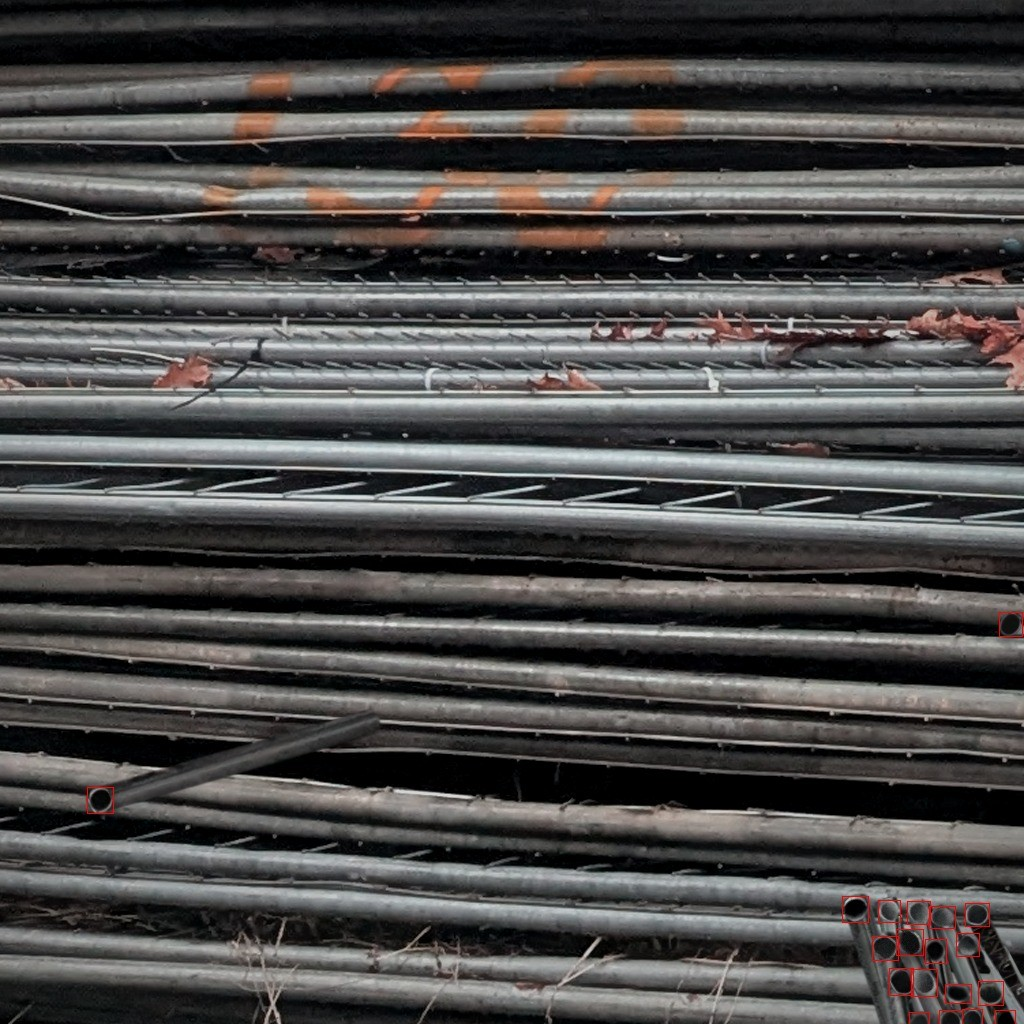
\includegraphics[width=\textwidth]{abbildungen/synth_000.jpg}
\end{subfigure}\hfill
\begin{subfigure}{0.245\textwidth}
  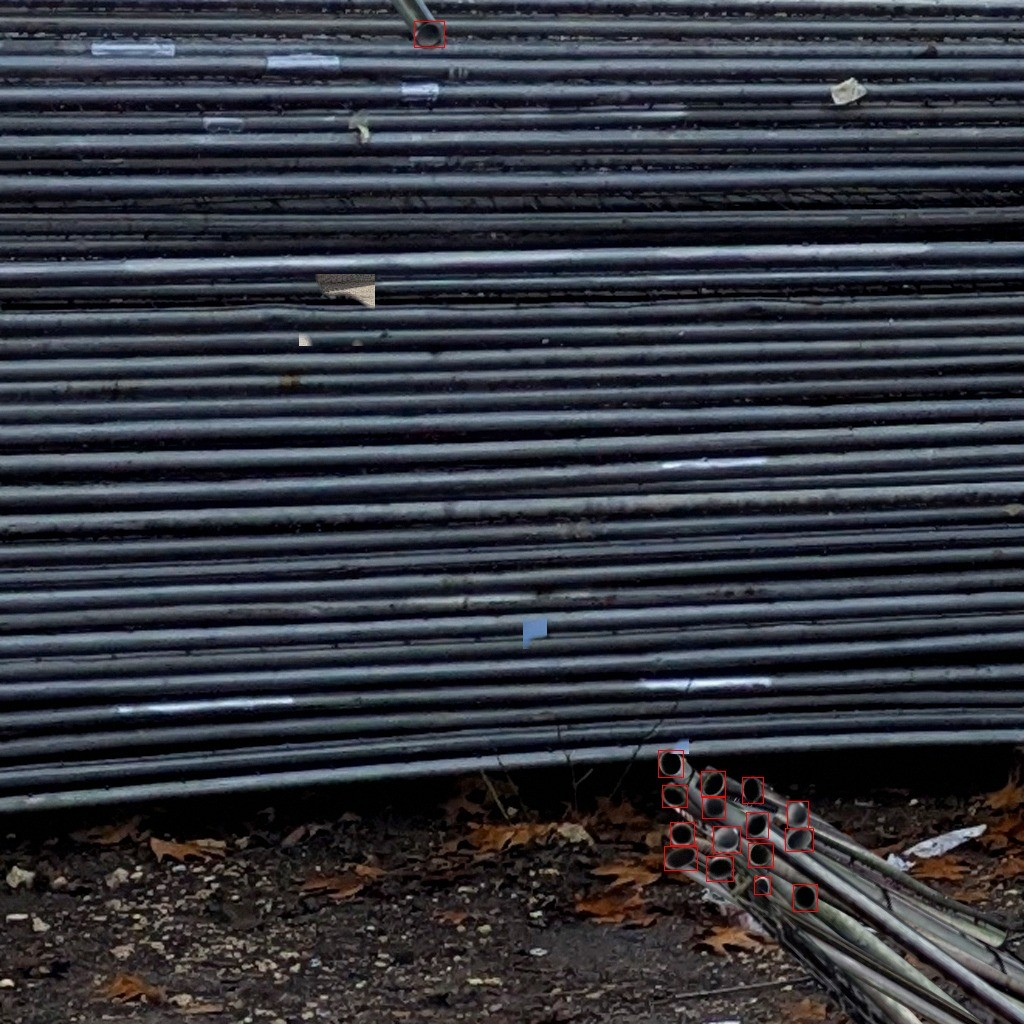
\includegraphics[width=\textwidth]{abbildungen/synth_001.jpg}
\end{subfigure}\hfill
\begin{subfigure}{0.245\textwidth}
  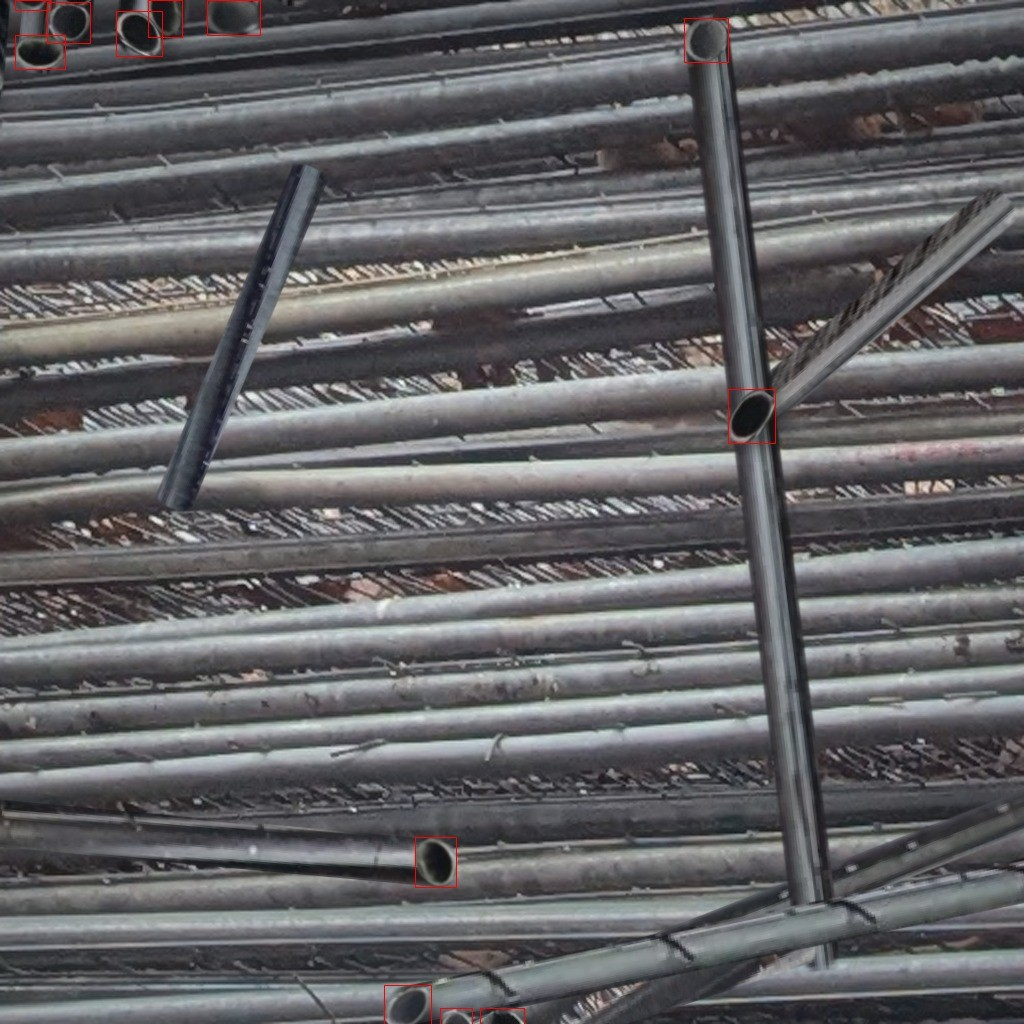
\includegraphics[width=\textwidth]{abbildungen/synth_003.jpg}
\end{subfigure}\hfill
\begin{subfigure}{0.245\textwidth}
  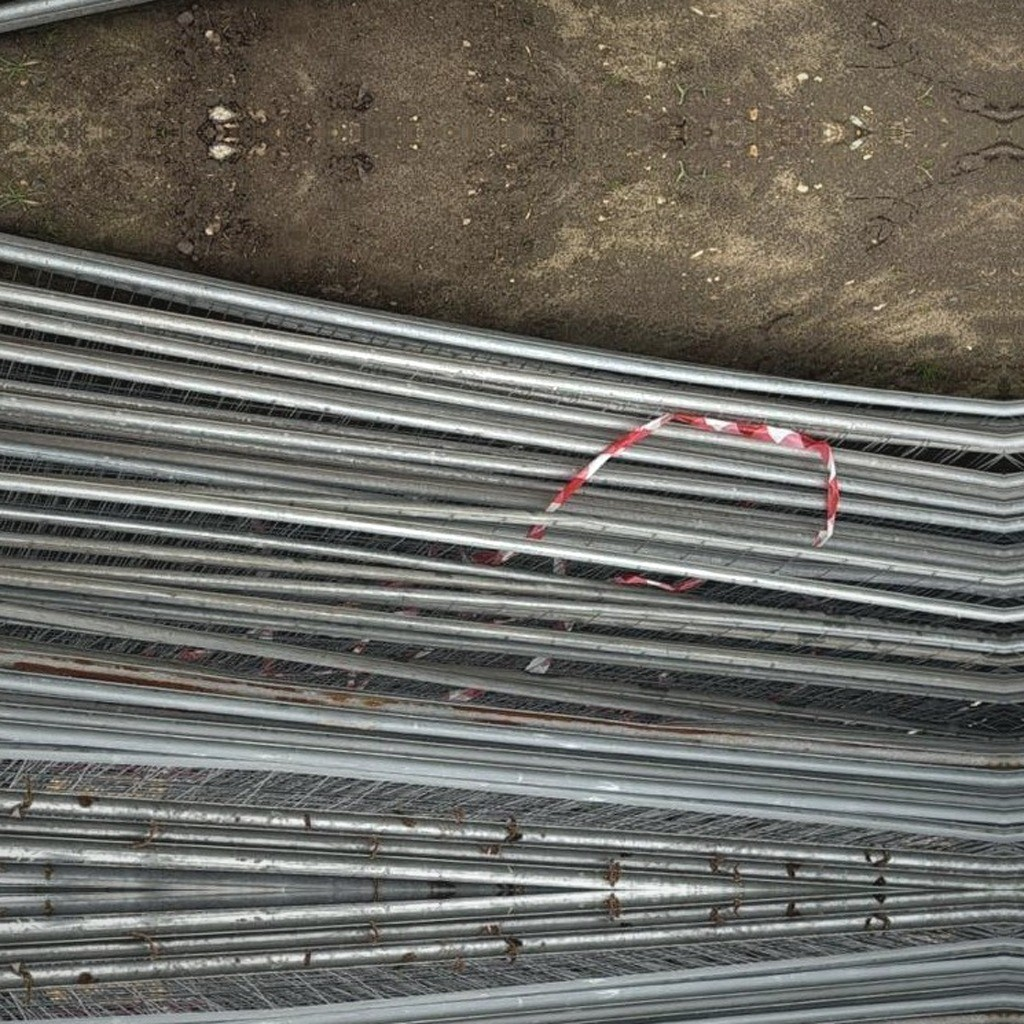
\includegraphics[width=\textwidth]{abbildungen/synth_004.jpg}
\end{subfigure}
\caption[Beispiele synthetischer Trainingsbilder]{Vier synthetische
Trainingsbilder mit den erzeugten Labels. Erkennbar sind die Clusterstruktur des
Layoutmodells, die Rohrschäfte hinter den Stirnflächen, die quer liegenden
Okkluder und die abgedunkelten Mulden.}
\label{abb:synthbeispiele}
\end{figure}

\begin{figure}[htbp]
\centering
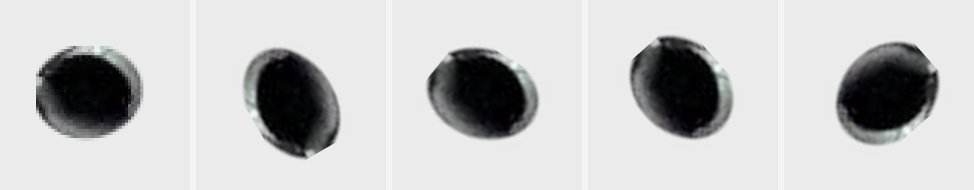
\includegraphics[width=\textwidth]{abbildungen/stufe_T2_geometrie.png}

\vspace{6pt}
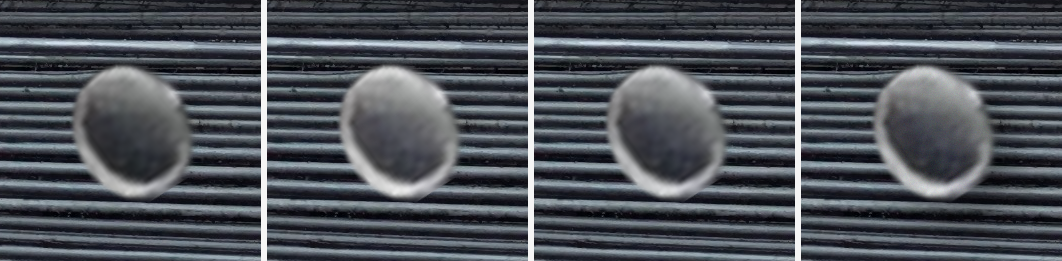
\includegraphics[width=\textwidth]{abbildungen/stufe_T3_photometrie.png}
\caption[Instanzgeometrie und Photometrie im Detail]{Die Stufen T2 und T3,
vergrößert. \emph{Oben (T2 Instanzgeometrie),
von links nach rechts:} der Quellausschnitt und vier Ziehungen aus $p(t)$ --
Rotation über den vollen Kreis, Skalierung, Ovalisierung, Delle, Perspektive.
Alle fünf Kacheln zeigen dasselbe Objekt bei gleichem Durchmesser.
\emph{Unten (T3 Photometrie), von links nach rechts:} dieselbe Instanz auf
demselben Hintergrund -- roh eingefügt, dann mit Photometrie, dann mit
Farbangleich, dann mit Einbettung und Schlagschatten. Der Farbangleich nach
Gleichung~\eqref{eq:harmonize} verschiebt die Verteilung nur teilweise; die
Einbettung ergänzt Kantenweichzeichnung, Rauschangleich nach
Gleichung~\eqref{eq:noise} und Schlagschatten. Für die Darstellung ist der
Zieldurchmesser auf 100\px{} gesetzt; im Datensatz liegt er bei 12--44\px.
Erzeugt mit \code{paper/tools/fig\_stufen.py}.}
\label{abb:stufendetail}
\end{figure}

\begin{figure}[htbp]
\centering
\begin{subfigure}{0.62\textwidth}
  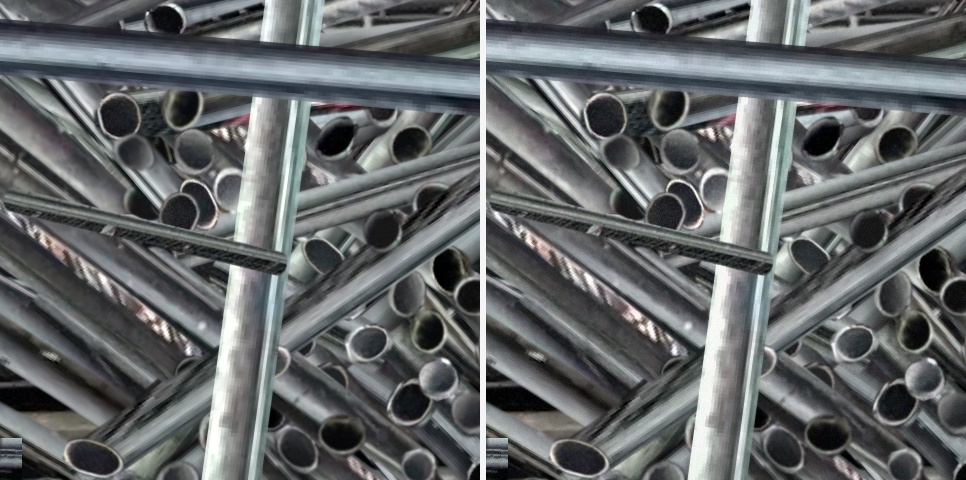
\includegraphics[width=\textwidth]{abbildungen/stufe_T8_global.jpg}
  \caption{T8 globale Bildstufe}
\end{subfigure}\hfill
\begin{subfigure}{0.35\textwidth}
  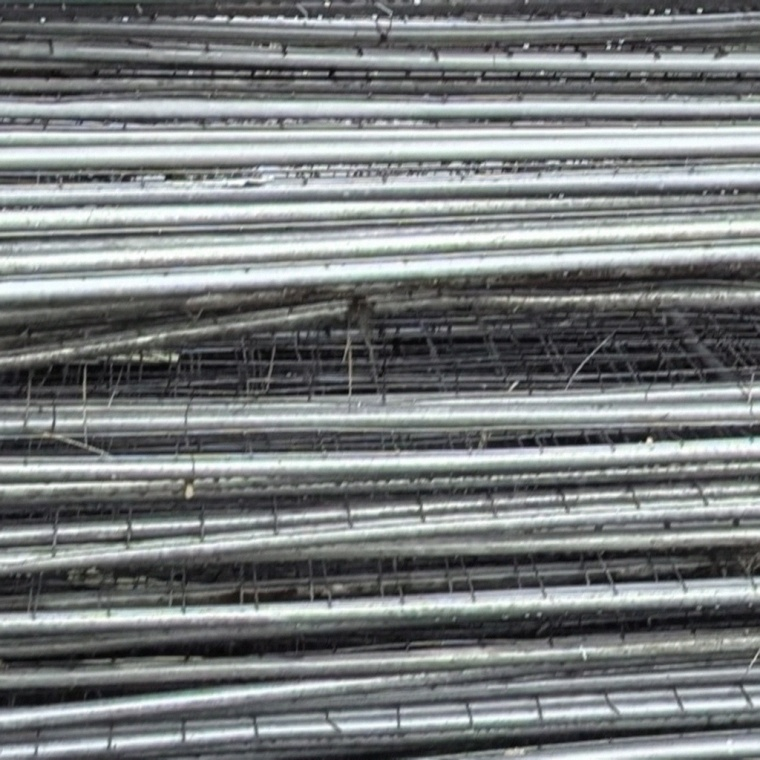
\includegraphics[width=\textwidth]{abbildungen/stufe_T9_negativ.jpg}
  \caption{T9 Negativbild}
\end{subfigure}
\caption[Globale Bildstufe und Negativbild]{Die Stufen T8 und T9.
(a)~Derselbe Bildausschnitt links ohne, rechts mit der globalen Stufe:
Helligkeit und
Kontrast, HSV, Defokus, Bewegungsunschärfe, Rauschen, Vignettierung und
JPEG-Requantisierung wirken auf das \emph{fertige} Bild und damit auf
eingefügte und originale Pixel gleichermaßen -- das ist ihr Zweck, denn ein
Unterschied in genau diesen Größen wäre eine Abkürzung im Sinne von
Tabelle~\ref{tab:signaturen}. (b)~Ein Negativbild: 9,7\,\% der Bilder enthalten
kein einziges Objekt. Gezeigt ist der schwierige Fall -- ein Rohrstapel
\emph{ohne} sichtbare Stirnflächen, also genau der Kontext, in dem Fehlalarme
entstehen. Erzeugt mit \code{paper/tools/fig\_stufen.py}.}
\label{abb:stufenglobal}
\end{figure}

\begin{figure}[htbp]
\centering
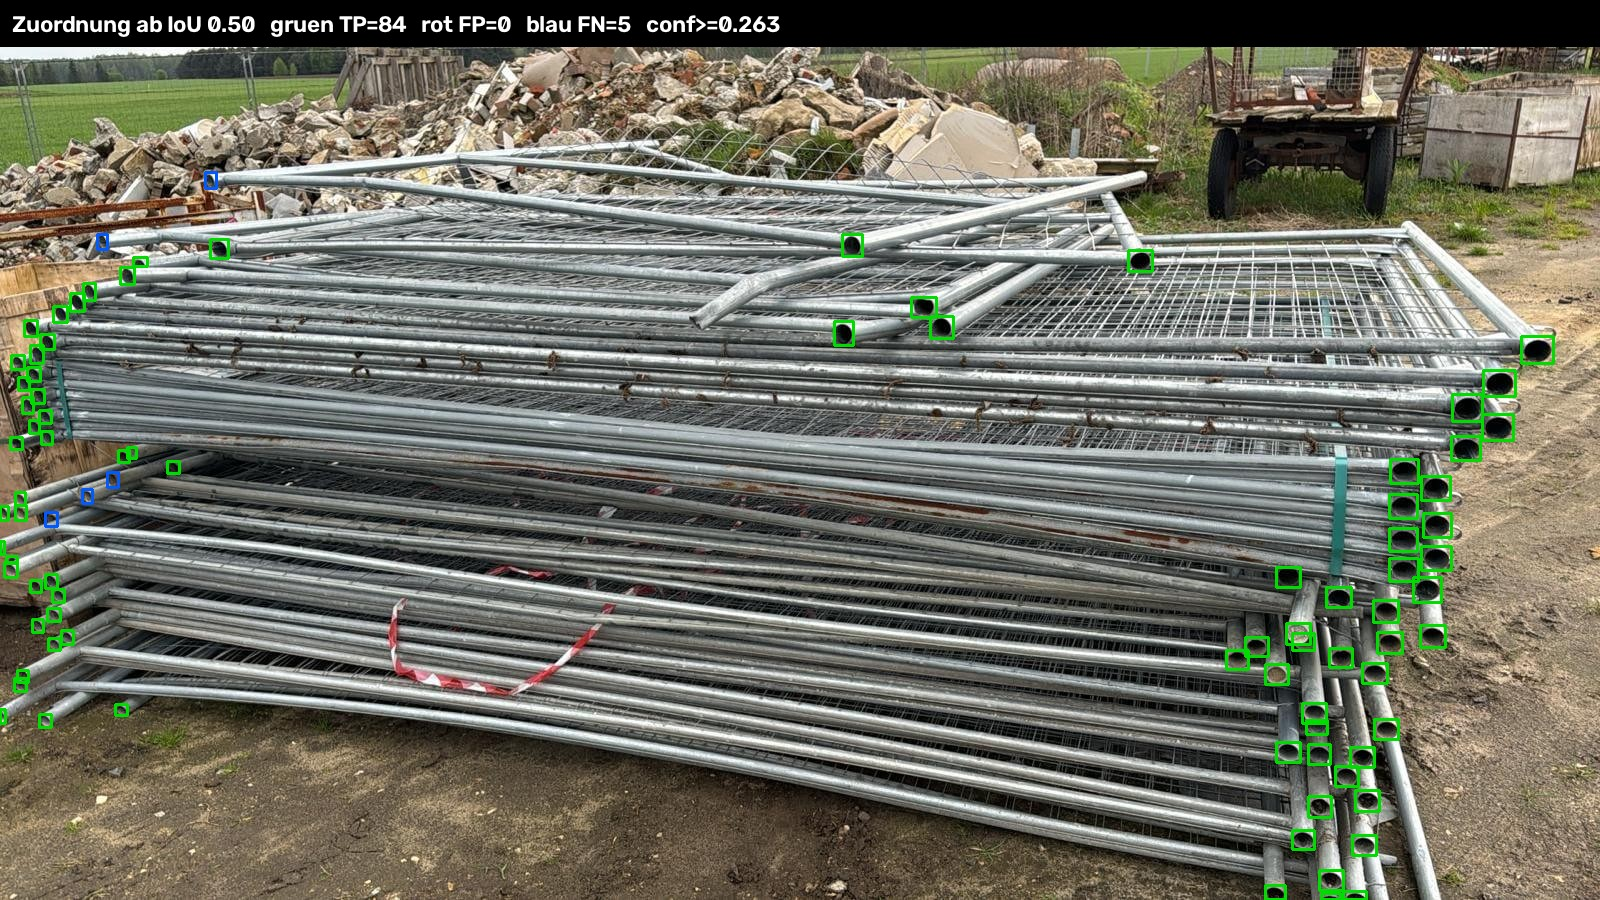
\includegraphics[width=0.93\textwidth]{abbildungen/qual_test_iou050.jpg}
\caption[Qualitatives Ergebnis auf \code{test}]{Qualitatives Ergebnis auf
\code{test} bei der berichteten Zuordnungsschwelle
$\mathrm{IoU} \geq 0{,}50$ \parencite{everingham2010,lin2014coco} und am
$F_1$-optimalen Betriebspunkt $c^* = 0{,}263$. Grün = Treffer, rot =
Falsch-Positiv, blau = Falsch-Negativ. Von 89 annotierten Stirnflächen werden
\textbf{84 getroffen, keine einzige Detektion ist falsch positiv}; die fünf
Falsch-Negativen liegen am linken Bildrand und am oberen Stapelrand, also bei
den kleinsten Objekten der Aufnahme. Erzeugt mit
\code{paper/tools/fig\_qual\_iou.py}.}
\label{abb:qualitativ}
\end{figure}

